\documentclass[tikz]{standalone}
\usepackage{pgfplots}
\pgfplotsset{compat=1.15}
\usepackage{mathrsfs}
\usetikzlibrary{arrows,calc}
\usepackage{tkz-euclide}

\pagestyle{empty}

\definecolor{AngleClr}{rgb}{0,0.39215686274509803,0}
\definecolor{BlueAngleClr}{HTML}{4e8fc2}
\definecolor{YellowAngleClr}{HTML}{b3a73e}
\definecolor{ShapeClr}{rgb}{0.6,0.2,0}
\definecolor{DarkGreekCircleClr}{HTML}{316614}

\begin{document}

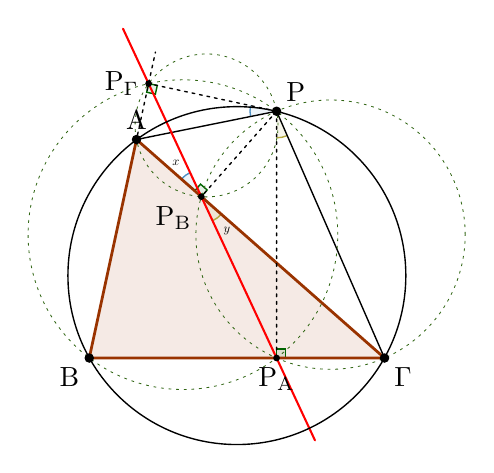
\begin{tikzpicture}[scale=.75]
\tkzSetUpLine[line width=1pt,color=black]
\tkzSetUpPoint[fill=black]

\tkzDefPoints{0/0/B,0.8/3.7/A,5/0/C}

\tkzDefTriangleCenter[circum](A,B,C) \tkzGetPoint{O}
\tkzDefPointBy[rotation=center O angle -50](A) \tkzGetPoint{P}

\tkzFillPolygon[fill=ShapeClr,fill opacity=0.1](A,B,C)

\tkzDefPointBy[projection = onto B--C](P) \tkzGetPoint{PA}
\tkzDefPointBy[projection = onto A--C](P) \tkzGetPoint{PB}
\tkzDefPointBy[projection = onto A--B](P) \tkzGetPoint{PC}


\tkzMarkAngles[line width=0.5pt, size=.45,color=BlueAngleClr](PC,P,A PC,PB,A)
\tkzFillAngles[line width=0.5pt, size=.45,fill=BlueAngleClr,fill opacity=0.1](PC,P,A PC,PB,A)
\tkzLabelAngle[scale=0.45,pos=1.6](PC,PB,A){$x$}

\tkzMarkAngles[line width=0.5pt, size=.45,color=YellowAngleClr](PA,PB,C PA,P,C)
\tkzFillAngles[line width=0.5pt, size=.45,fill=YellowAngleClr,fill opacity=0.1](PA,PB,C PA,P,C)
\tkzLabelAngle[scale=0.45,pos=1.6](PA,PB,C){$y$}

\tkzMarkRightAngles[line width=0.5pt, size=.15,color=AngleClr,fill=AngleClr,fill opacity=0.1](P,PA,C P,PB,A P,PC,B)

\tkzDrawSegments[line width=0.5pt,color=black,dashed,dash pattern=on 1pt off 1.75pt,add=0 and 0.4](B,A)
\tkzDrawPolygon[color=ShapeClr](A,B,C)


\tkzDrawSegments[line width=0.5pt,color=black](P,A P,C)
\tkzDrawSegments[line width=0.5pt,color=black,dashed,dash pattern=on 1pt off 1.75pt](P,PA P,PB P,PC)
\tkzDrawSegments[line width=0.75pt,color=red,add=0.3 and 0.2](PA,PC)

\tkzDrawCircle[color=black,line width=0.5pt](O,A)

\tkzDefTriangleCenter[circum](P,PB,PC) \tkzGetPoint{OA}
\tkzDefTriangleCenter[circum](P,PA,PC) \tkzGetPoint{OB}
\tkzDefTriangleCenter[circum](P,PA,PB) \tkzGetPoint{OC}

\tkzDrawCircles[color=DarkGreekCircleClr,line width=0.3pt, dashed,dash pattern=on 1pt off 1.75pt](OA,P OB,P OC,P)

\tkzDrawPoints[size=3](A,B,C,P)
\tkzDrawPoints[size=2](PA,PB,PC)
\tkzLabelPoint[above](A){$\rm A$}
\tkzLabelPoint[below left](B){$\rm B$}
\tkzLabelPoint[below right](C){$\rm \Gamma$}

\tkzLabelPoint[below](PA){$\rm P_A$}
\tkzLabelPoint[below left](PB){$\rm P_B$}
\tkzLabelPoint[left](PC){$\rm P_\Gamma$}
\tkzLabelPoint[above right](P){$\rm P$}

\end{tikzpicture}

\end{document}
